\documentclass[a4,openany,landscape,tikz]{article}
%\documentclass[11pt,a5,landscape,openany]{article}
\usepackage{xcolor}
\usepackage{makeidx}
\usepackage{geometry}       
\usepackage[chorded]{songs} 
\usepackage[colorlinks=true, pdfstartview=FitV, linkcolor=blue, citecolor=blue, urlcolor=blue]{hyperref} 
\usepackage{fancyhdr}
%\usepackage{abc}
%\usepackage{lilypond}
%\usepackage[parfill]{parskip}  
\usepackage{graphicx}
\usepackage{wrapfig}
\usepackage{qrcode}
%\usepackage{amssymb}
%\usepackage{epstopdf}
%\DeclareGraphicsRule{.tif}{png}{.png}{`convert #1 `dirname #1`/`basename #1 .tif`.png}

\usepackage{tikz}
\usetikzlibrary{decorations.text}


\setlength{\topmargin}{-0.5cm}
\setlength{\headheight}{0cm}
\setlength{\headsep}{-0.5cm}
\setlength{\textheight}{18cm}
\setlength{\textwidth}{24cm}
\setlength{\oddsidemargin}{-0.5cm}
\setlength{\evensidemargin}{-0.5cm}	
\setlength{\parindent}{0.25cm}
%\setlength{\parskip}{0.25cm}


\songpos{2}

%\pagestyle{fancy}
%\fancyhf{}
%\lfoot{%
%	\begin{minipage}{\textwidth}
%	\parbox{0.46\linewidth}{Some text to go in the footer Some text to go in the footer}\hfill
%	\parbox{0.70\linewidth}{
\includegraphics[width=0.2\linewidth]{KK/KuylKamp_vierkantje_logo}}\hfill
%	\parbox{0.60\linewidth}{\raggedleft
\includegraphics[width=0.2\linewidth]{KK/KuylKamp_naam}}\hfill
%	\parbox{0.02\linewidth}{\raggedleft \thepage}%
%	\end{minipage}
%}

\renewcommand\printchord[1]{{\color{red!70!black}#1}}

\renewcommand{\songchapter}{\subsection}
\renewcommand{\songsection}{\subsection}

\newcommand{\U}{\Uparrow}
\newcommand{\D}{\Downarrow}


% ------------------- Title and Author -----------------------------
\title{AMeeSpeel KuylKampVuur Songbook 2016}

\author{gathered by Grobozeak-KKVO}
%\newindex{titleidx}{titleidx}
%\newauthorindex{authidx}{authidx}

%\frontmatter

\begin{document}
%\songcolumns{2}

\maketitle 

%\qrcode[hyperlink]{https://www.kuylkamp.nl}

%\parbox{0.70\linewidth}{
\includegraphics[width=0.2\linewidth]{KK/KuylKamp_vierkantje_logo}}\hfill

 
\begin{wrapfigure}{l}{0.20\textwidth}
\qrcode[hyperlink]{https://github.com/coentjo/songbooks/releases}

%\url{https://github.com/coentjo/songbooks/releases}. 
\end{wrapfigure}


Bij een aantal nummers is aangegeven op welke positie de capo moet staan om met het origineel mee te kunnen spelen (als je het bijvoorbeeld op youtube opzoekt). Op het KuylKamp zullen we zoveel mogelijk \emph{zonder} spelen.  

Dit songbook is ook te vinden op internet, verstopt achter de URL \url{https://github.com/coentjo/songbooks/releases}. 

Op die internetpagina staan ook een aantal links naar opnamen van een aantal nummers zoals ze ook in de map staan.  
Natuurlijk heb je een gestemde gitaar nodig. Als je geen stemmer hebt kun je je mobiel gebruiken met een app: Zoek in de app store van je keuze op `\emph{Guitar Tuner}'. Zelf heb ik goeie ervaringen met `PitchLab Guitar Tuner' onder Android. 

Fouten, wijzigingen of andere tips? Geef ze door via email:   \href{mailto:coentjo@gmail.com}{coentjo@gmail.com} 

\begin{wrapfigure}{l}{0.25\textwidth}

\includegraphics[width=0.3\linewidth]{KK/KuylKamp_vierkantje_logo} 
\end{wrapfigure}


\begin{tikzpicture}[mypostaction/.style 2 args={
                         decoration={
                              text align={
                                    left indent=#1},
                                    text along path, 
                                    text={#2}
                                    },
                           decorate
                        }
                    ]
  \coordinate (specRoot) at (-10,0);
  \coordinate (testTreeRoot) at (0,0);
  \draw[-latex, blue!20!white, line width=5ex]  (specRoot) to[in=135,out=45] (testTreeRoot);

  \path [postaction={mypostaction={1cm}{Sla snel de bladzijde om}},
         postaction={mypostaction={1cm}{en begin met spelen!},
         /pgf/decoration/raise=-3mm}]
    (specRoot) to [in=120,out=45] (testTreeRoot);
\end{tikzpicture}

%\url{https://github.com/coentjo/songbooks/releases/download/v0.1/Amy_Green.Day.mp3}
%\qrcode{https://github.com/coentjo/songbooks/releases/download/v0.1/Amy_Green.Day.mp3}


%\tableofcontents 
%\showindex{Al hun liedjes}{titleidx}

%\showindex[2]{Nummers}{titleidx}
%\showindex[2]{artiesten}{authidx}


%\begin{abc}[name=c-dur]
%X: 1 % start of header
%K: C % scale: C major
%"Text"C4 G4 | (3FED c4 G2 |
%\end{abc}
%\newpage

\begin{songs}{} %{titleidx,authidx}

	\songcolumns{2}


	% Activate the following line by filling in the right side. If for example the name of the root file is Main.tex, write
% "...root = Main.tex" if the chapter file is in the same directory, and "...root = ../Main.tex" if the chapter is in a subdirectory.
 
%!TEX root = ../boktor.tex 

\beginsong{The wild rover}[by=Dubliners]
%\capo{3}
\begin{LARGE}
\ \\
Ritme (3/4): $ \D . \ . \U \D \U $ \\
\ \\
\end{LARGE}

%{\nolyrics Intro: \[E] \[G] \[A]}

\gtab{G}{320003}
\gtab{C}{332010}
\gtab{D7}{XX0232}



\beginverse
I've \[G]been a wild rover for many a \[C]year
I \[G]spent all me \[C]money on \[D7]whiskey and \[G]beer
But \[G]now I'm returning with gold in great \[C]store
And I \[G]never will \[C]play the wild \[D7]rover no \[G]more
\endverse



\beginchorus
  And it's \[D7]no nay never, \brk  \[klop klop klop] \[G]  \brk  no nay never no \[C]more
  Will I \[G]play the wild \[C]rover, no \[D7]never, no \[G]more
\endchorus



\beginverse
I \[G]went in to an alehouse I used to \[C]frequent
And I \[G]told the land\[C]lady me \[D7]money was \[G]spent
I \[G]asked her for credit, she answered me \[C]`Nay!'
`Such \[G]custom as \[C]yours I could \[D7]have any \[G]day!'
\endverse



\beginchorus
  And it's \[D7]no nay never, \brk  \[klop klop klop] \[G]  \brk  no nay never no \[C]more
  Will I \[G]play the wild \[C]rover, no \[D7]never, no \[G]more
\endchorus



\beginverse
I \[G]took out of me pocket ten sovereigns \[C]bright
And the \[G]landlady's \[C]eyes opened \[D7]wide with de\[G]light
She \[G]said: `I have whiskeys and wines on the \[C]best!
And the \[G]words that I \[C]told you were \[D7]only in \[G]jest!'
\endverse



\beginchorus
  And it's \[D7]no nay never, \brk  \[klop klop klop] \[G]  \brk  no nay never no \[C]more
  Will I \[G]play the wild \[C]rover, no \[D7]never, no \[G]more
\endchorus



\beginverse
I'll go \[G]home to my parents, confess what I've \[C]done
And \[G]ask them to \[C]pardon their \[D7]prodigal \[G]son
And \[G]when they've caressed me as oftimes be\[C]fore
I \[G]never will \[C]play the wild \[D7]rover no \[G]more.
\endverse

%\beginverse
%\endverse


\beginchorus
	(2x)
  And it's \[D7]no nay never, \brk  \[klop klop klop] \[G]  \brk  no nay never no \[C]more
  Will I \[G]play the wild \[C]rover, no \[D7]never, no \[G]more
\endchorus



\endsong
					
	
		\beginscripture{(had een oud Chinees spreekwoord kunnen zijn)}
			Beter elke dag 5 minuten met in de hand een gitaar,
			
			Dan eenmaal per week een uur, 't is echt waar!
		\endscripture	
		
	
	% Activate the following line by filling in the right side. If for example the name of the root file is Main.tex, write
% "...root = Main.tex" if the chapter file is in the same directory, and "...root = ../Main.tex" if the chapter is in a subdirectory.
 
%!TEX root = ../songbook.tex 

\beginsong{wonderwall }[by=Oasis]
\capo{3 voor originele hoogte, maar Kuylkamp: zonder capo} 

\begin{LARGE} 
Ritme: $ \D . \D . \D \U \D \U $  \\
\ \\
\end{LARGE} 


\gtab{Ex}{022033}
\gtab{Gx}{320033}
\gtab{Dx}{000233}
\brk
\gtab{Ax}{002033}
\gtab{Cx}{X32033}
\gtab{F#x}{200233}


\beginverse
{\nolyrics Intro (2x): \[ Ex Gx Dx Ax ] }
\endverse


\beginverse
\[Ex] Today is \[Gx]gonna be the day,   \brk   That they're \[Dx]gonna throw it back to \[Ax]you
\[Ex] By now you \[Gx]should've somehow,   \brk   Rea\[Dx]lized what you gotta \[Ax]do
\[Ex]I don't believe that \[Gx]anybody,   \brk   \[Dx]Feels the way I \[Ax]do about you \[Ex]now \[Gx] \[Dx] \[Ax]
\endverse

\beginverse
\[Ex] Backbeat the \[Gx]word was on the street,   \brk   That the \[Dx]fire in your heart is \[Ax]out
\[Ex] I'm sure you've \[Gx]heard it all before,   \brk   But you \[Dx]never really had a \[Ax]doubt
\[Ex]I don't believe that \[Gx]anybody,   \brk   \[Dx]Feels the way I \[Ax]do about you \[Ex]now \[Gx] \[Dx] \[Ax]
\endverse

\beginchorus
And \[Cx]all the roads we \[Dx]have to walk are \[Ex]winding \[Ex]
And \[Cx]all the lights that \[Dx]lead us there are \[Ex]blinding  \[Ex]
\[Cx]There are many \[Dx]things that I would \[Gx]like to \[F#x]say to \[Ex]you,   \brk But I don't know \[Dx]how  \[Ax]
\endchorus

\beginchorus
Because \[Cx]maybe  \[Ex] \[Gx],   \brk   You're \[Ex]gonna be the one that \[Cx]saves me \[Ex]  \[Gx]
And \[Ex]after all\[Cx]  \[Ex] \[Gx],   \brk   You're my \[Ex]wonderwall \[Cx]  \[Ex] \[Gx]
\endchorus

\beginverse
\[Ex] Today was \[Gx]gonna be the day,   \brk   But they'll \[Dx]never throw it back to \[Ax]you
\[Ex] By now you \[Gx]should've somehow,   \brk   Rea\[Dx]lized what you're not to \[Ax]do
\[Ex]I don't believe that \[Gx]anybody,   \brk   \[Dx]Feels the way I \[Ax]do about you \[Ex]now \[Gx] \[Dx] \[Ax]
\endverse

\beginchorus
And \[Cx]all the roads we \[Dx]have to walk are \[Ex]winding \[Ex]
And \[Cx]all the lights that \[Dx]lead us there are \[Ex]blinding
\[Cx]There are many \[Dx]things that I would \[Gx]like to \[F#x]say to \[Ex]you,   \brk   But I don't know \[Dx]how  \[Ax]
\endchorus

\beginchorus
\rep{2}
I said \[Cx]maybe \[Ex] \[Gx] ,   \brk   You're \[Ex]gonna be the one that \[Cx]saves me \[Ex] \[Gx] 
And \[Ex]after \[Cx]all \[Ex] \[Gx] ,   \brk   You're my \[Ex]wonderwall  \[ Cx Ex Gx Ex ]
\endchorus

\beginchorus
I said \[Cx]maybe \[Ex] \[Gx] 
\rep{3}  You're \[Ex]gonna be the one that \[Cx]saves me \[Ex] \[Gx] 
\endchorus

\textnote{de akkoordnamen met `x' zijn niet de echte namen... maar die hebben veel te moeilijke namen...}
\endsong
    \setcounter{songnum}{2}
	% Activate the following line by filling in the right side. If for example the name of the root file is Main.tex, write
% "...root = Main.tex" if the chapter file is in the same directory, and "...root = ../Main.tex" if the chapter is in a subdirectory.
 
%!TEX root = ../songbook.tex 

\beginsong{wonderwall }[by=Oasis]
\capo{3 voor originele hoogte, maar Kuylkamp: zonder capo} 

%\begin{LARGE} 
%Ritme: $ \D . \D . \D \U \D \U $  \\
%\ \\
%\end{LARGE} 


\gtab{Em7}{022033}
\gtab{G}{320033}
\gtab{Dsus4}{000233}
\brk
\gtab{Ax}{002033}
\gtab{Cadd9}{X32033}
\gtab{G/F#}{200233}


\beginverse
{\nolyrics Intro (2x): \[ Em7 G Dsus4 Ax ] }
\endverse


\beginverse
\[Em7] Today is \[G]gonna be the day,   \brk   That they're \[Dsus4]gonna throw it back to \[Ax]you
\[Em7] By now you \[G]should've somehow,   \brk   Rea\[Dsus4]lized what you gotta \[Ax]do
\[Em7]I don't believe that \[G]anybody,   \brk   \[Dsus4]Feels the way I \[Ax]do about you \[Em7]now \[G] \[Dsus4] \[Ax]
\endverse

\beginverse
\[Em7] Backbeat the \[G]word was on the street,   \brk   That the \[Dsus4]fire in your heart is \[Ax]out
\[Em7] I'm sure you've \[G]heard it all before,   \brk   But you \[Dsus4]never really had a \[Ax]doubt
\[Em7]I don't believe that \[G]anybody,   \brk   \[Dsus4]Feels the way I \[Ax]do about you \[Em7]now \[G] \[Dsus4] \[Ax]
\endverse

\beginchorus
And \[Cadd9]all the roads we \[Dsus4]have to walk are \[Em7]winding \[Em7]
And \[Cadd9]all the lights that \[Dsus4]lead us there are \[Em7]blinding  \[Em7]
\[Cadd9]There are many \[Dsus4]things that I would \[G]like to \[G/F#]say to \[Em7]you,   \brk But I don't know \[Dsus4]how  \[Ax]
\endchorus

\beginchorus
Because \[Cadd9]maybe  \[Em7] \[G],   \brk   You're \[Em7]gonna be the one that \[Cadd9]saves me \[Em7]  \[G]
And \[Em7]after all\[Cadd9]  \[Em7] \[G],   \brk   You're my \[Em7]wonderwall \[Cadd9]  \[Em7] \[G]
\endchorus

\beginverse
\[Em7] Today was \[G]gonna be the day,   \brk   But they'll \[Dsus4]never throw it back to \[Ax]you
\[Em7] By now you \[G]should've somehow,   \brk   Rea\[Dsus4]lized what you're not to \[Ax]do
\[Em7]I don't believe that \[G]anybody,   \brk   \[Dsus4]Feels the way I \[Ax]do about you \[Em7]now \[G] \[Dsus4] \[Ax]
\endverse

\beginchorus
And \[Cadd9]all the roads we \[Dsus4]have to walk are \[Em7]winding \[Em7]
And \[Cadd9]all the lights that \[Dsus4]lead us there are \[Em7]blinding
\[Cadd9]There are many \[Dsus4]things that I would \[G]like to \[G/F#]say to \[Em7]you,   \brk   But I don't know \[Dsus4]how  \[Ax]
\endchorus

\beginchorus
I said \[Cadd9]maybe \[Em7] \[G] ,   \brk   You're \[Em7]gonna be the one that \[Cadd9]saves me \[Em7] \[G] 
And \[Em7]after \[Cadd9]all \[Em7] \[G] ,   \brk   You're my \[Em7]wonderwall  \[ Cadd9 Em7 G Em7 ]
\endchorus

\beginchorus
I said \[Cadd9]maybe \[Em7] \[G] ,   \brk   You're \[Em7]gonna be the one that \[Cadd9]saves me \[Em7] \[G] 
And \[Em7]after \[Cadd9]all \[Em7] \[G] ,   \brk   You're my \[Em7]wonderwall  \[ Cadd9 Em7 G Em7 ]
\endchorus

\beginchorus
I said \[Cadd9]maybe \[Em7] \[G] 
\rep{3}  You're \[Em7]gonna be the one that \[Cadd9]saves me \[Em7] \[G] 
\endchorus

\endsong
 
	% Activate the following line by filling in the right side. If for example the name of the root file is Main.tex, write
% "...root = Main.tex" if the chapter file is in the same directory, and "...root = ../Main.tex" if the chapter is in a subdirectory.
 
%!TEX root = ../boktor.tex 

\beginsong{Brown eyed girl }[by=Van Morrison]


\begin{LARGE} 
Ritme: $ \D . \D \U . \ . \D . $  \\
\end{LARGE} 


\gtab{G}{320003}
\gtab{C}{332010}
\gtab{D}{XX0232}
\gtab{E}{022100}



\beginverse
\[G] Hey, where did we \[C]go,   \brk   \[G] Days when the \[D]rain came
\[G] Down in the \[C]hollow,   \brk   \[G] Playing a \[D]new game
\[G] Laughing, and a \[C]running, hey hey,   \brk   \[G] Skipping and a \[D]jumping
\[G] In the misty \[C]morning fog with,   \brk   \[G] Our \[D]hearts a thumpin' and \[C]you
\[D] My brown eyed \[G]girl  \[Em],   \brk   \[C] You\[D], my brown eyed \[G]girl \[D]
\endverse


\beginverse
\[G] Whatever \[C]happened ,   \brk   to \[G] Tuesday and \[D]so slow
\[G] Going down the \[C]old mine with a ,   \brk   \[G] transistor \[D]radio
\[G] Standing in the \[C]sunlight laughing,   \brk   \[G] Hiding behind a \[D]rainbow's wall
\[G] Slipping and a \[C]sliding,   \brk   \[G] All along the \[D]waterfall, with \[C]you
\[D] My brown eyed \[G]girl  \[Em],   \brk   \[C] You\[D], my brown eyed \[G]girl \[D]
\endverse

\beginchorus
\[D]Do you remember when we used to \[G]sing
Sha la la \[C]la la la la \[G]la la la la te \[D]da   Just like \[G]that
Sha la la \[C]la la la la \[G]la la la la te \[D]da   La te \[G]da
\endchorus


\beginverse
((( BASS SOLO )))
\endverse


\beginverse
\[G] So hard to \[C]find my way,   \brk   \[G] Now that I'm \[D]all on my own
\[G] I saw you just the \[C]other day,   \brk   \[G] My, how \[D]you have grown
\[G] Cast my memory \[C]back there Lord,   \brk   \[G] Sometimes I'm \[D]overcome thinkin' 'bout
\[G] Making love in the \[C]green grass,   \brk   \[G] Behind the \[D]stadium, with \[C]you \[D]
My brown eyed \[G]girl \[Em],   \brk   \[C]You\[D], my brown eyed \[G]girl
\endverse

\beginchorus
\[D]Do you remember when we used to \[G]sing
(4x) Sha la la \[C]la la la la \[G]la la la la te \[D]da   Just like \[G]that
\endchorus



\endsong
 
	% Activate the following line by filling in the right side. If for example the name of the root file is Main.tex, write
% "...root = Main.tex" if the chapter file is in the same directory, and "...root = ../Main.tex" if the chapter is in a subdirectory.
 
%!TEX root = ../boktor.tex 

\beginsong{Country Roads}[by=John Denver]


\gtab{G}{320003}
\gtab{Em}{022000}
\gtab{D}{XX0232}
\gtab{D7}{XX0212}
\gtab{C}{332010}
\gtab{F}{133211}

\beginverse
{\nolyrics Intro: \[G] }
\endverse

\memorize
\beginverse
\[G] Almost heaven, \[Em]West Virginia
\[D]Blue ridge mountains, \[C]Shenandoah \[G]river
\[G]Life is old there, \[Em]older than the trees
\[D]Younger than the mountains, \[C]growin' like a \[G]breeze
\endverse

\beginchorus
Country \[G]roads, take me \[D]home
To the \[Em]place I be\[C]long
West Vir\[G]ginia, mountain \[D]momma
Take me \[C]home, country \[G]roads
\endchorus

\beginverse
^ All my memories, ^gather 'round her
^Miner's lady, ^stranger to blue ^water
^Dark and dusty, ^painted on the sky
^Misty taste of moonshine, ^teardrops in my ^eyes
\endverse

\beginchorus
Country \[G]roads, take me \[D]home
To the \[Em]place I be\[C]long
West Vir\[G]ginia, mountain \[D]momma
Take me \[C]home, country \[G]roads
\endchorus

\beginverse
\[Em] I hear her \[D]voice in the \[G]mornin' hour she calls me
\[C]Radio re\[G]minds me of my \[D]home far away
\[Em]Drivin' down the \[F]road I get a \[C]feelin'
That I should have been home \[D]yesterday, \[D7]yesterday
\endverse

\beginchorus
\rep{2}
Country \[G]roads, take me \[D]home
To the \[Em]place I be\[C]long
West Vir\[G]ginia, mountain \[D]momma
Take me \[C]home, country \[G]roads
\endchorus

\beginchorus
\rep{2}: Take me \[D7]home, country \[G]roads
\endchorus


\endsong
					
	% Activate the following line by filling in the right side. If for example the name of the root file is Main.tex, write
% "...root = Main.tex" if the chapter file is in the same directory, and "...root = ../Main.tex" if the chapter is in a subdirectory.
 
%!TEX root = ../boktor.tex 

\beginsong{House of the rising sun}[]


\gtab{Am}{002210}
\gtab{C}{332010}
\gtab{D}{XX0232}
\gtab{F}{133211}
\gtab{E7}{020100}


\beginverse
There \[Am]is a \[C]house in \[D]New Or\[F]leans,
They \[Am]call the `\[C]Rising \[E7]Sun' \[E7],
It's \[Am]been the \[C]ruin of \[D]many a poor \[F]boy
And \[Am]God, I \[E7]know, I'm \[Am]one \[C D F Am E7 Am E7].
\endverse

\beginverse
My m^other ^was a t^ailor ^ ,
She s^ewed my n^ew blue j^eans ^,
My f^ather w^as a g^ambling m^an,
d^own in N^ew Orl^eans ^    .
\endverse

\beginverse
Now the ^only ^thing a ^gambler ^needs
is a ^suitcase ^and a ^trunk  ^
and the ^only ^time he'll be ^satis^fied
is ^when he's ^all a ^drunk ^  .
\endverse

\beginverse
Oh, ^mother, ^ tell your ^children ^
Not to ^do what ^I have ^done ^-
^Spend your ^lives in ^sin and mise^ry
In the ^House of ^Rising Sun ^ ^
\endverse

\beginverse
Well, I ^got one ^foot on the ^platform ^,
The ^other's ^on the ^train ^,
I'm ^going ^back to ^New Or^leans,
to ^wear that ^ball and ^chain ^ .
\endverse

\beginverse
There \[Am]is a \[C]house in \[D]New Or\[F]leans,
They \[Am]call the `\[C]Rising \[E7]Sun' \[E7],
It's \[Am]been the \[C]ruin of \[D]many a poor \[F]boy
And \[Am]God, I \[E7]know, I'm \[Am]one \[C D F Am E7 Am E7].
\endverse



\endsong
 
	% Activate the following line by filling in the right side. If for example the name of the root file is Main.tex, write
% "...root = Main.tex" if the chapter file is in the same directory, and "...root = ../Main.tex" if the chapter is in a subdirectory.

%!TEX root = ../boktor.tex

\beginsong{Where did you sleep Last Night?}[by=nirvana]


%{\nolyrics Intro: \[E] \[G] \[A]}


\beginverse
My girl, my girl, don't lie to me, Tell me where did you sleep last night
In the pines, in the pines, Where the sun don't ever shine,
I would shiver the whole night through
\endverse

\beginverse
My girl, my girl, where will you go, I'm going where the cold wind blows
In the pines, in the pines, Where the sun don't ever shine,
I would shiver the whole night through
\endverse

\beginverse
Her husband, was a hard working man, Just about a mile from here
His head was found in a driving wheel, But his body never was found
My girl, my girl, don't lie to me
Tell me where did you sleep last night
In the pines, in the pines, Where the sun don't ever shine,
I would shiver the whole night through
\endverse

\beginverse
- Zwischenspiel -
\endverse

\beginverse
My girl, my girl, where will you go, I'm going where the cold wind blows
In the pines, in the pines, Where the sun don't ever shine
I would shiver the whole night through
\endverse

\beginverse
My girl, my girl, don't lie to me
Tell me where did you sleep last night
In the pines, in the pines, Where the sun don't ever shine
I would shiver the whole night through
\endverse

\beginverse
My girl, my girl, where will you go, I'm going where the cold wind blows
In the pines, the pines, The sun shines
I'll shiver ... the whole night through
\endverse

\endsong
 
	% Activate the following line by filling in the right side. If for example the name of the root file is Main.tex, write
% "...root = Main.tex" if the chapter file is in the same directory, and "...root = ../Main.tex" if the chapter is in a subdirectory.
 
%!TEX root = ../boktor.tex 

%\begin[quote,fragment,staffsize=26]{lilypond}


%\begin{lilypond}
%c d e f 
%\end{lilypond}


\beginsong{Come as you are }[by=Nirvana]


%{\nolyrics Intro: \[E] \[G] \[A]}

\beginverse
Come as you are, as you were
As I want you to be
As a friend, as a friend
As an old enemy

Take your time, hurry up
The choice is yours, don't be late
Take a rest as a friend
As an old
\endverse

\beginchorus
Memoria, memoria
Memoria, memoria
\endchorus

\beginverse
Come doused in mud, soaked in bleach
As I want you to be
As a trend, as a friend
As an old
\endverse

\beginchorus
Memoria, memoria
Memoria, memoria
\endchorus

\beginverse
And I swear that I don't have a gun
No I don't have a gun
No I don't have a gun
\endverse

\beginchorus
Memoria, memoria
Memoria, memoria
(No I don't have a gun)

And I swear that I don't have a gun
No I don't have a gun
No I don't have a gun
No I don't have a gun
No I don't have a gun

Memoria, memoria
\endchorus



\endsong
 
	% Activate the following line by filling in the right side. If for example the name of the root file is Main.tex, write
% "...root = Main.tex" if the chapter file is in the same directory, and "...root = ../Main.tex" if the chapter is in a subdirectory.
 
%!TEX root = ../boktor.tex 

\beginsong{Zombie }[by=Cranberries]

\gtab{Em}{022000}
\gtab{C}{332010}
\gtab{G}{320003}
\gtab{D}{XX0232}

%{\nolyrics Intro: \[E] \[G] \[A]}

\beginverse
intro (4x): \ \[ Em Cmaj7 G D ]
\endverse


\memorize
\beginverse
\[Em] Another h\[C]ead hangs lowly,   \brk   Ch\[G]ild is slowly \[D]taken
\[Em]And the violence \[C]caused such silence,   \brk   \[G]Who are we mis\[D]taken

But you \[Em]see it's not me,   \brk   It's not \[C]my family
In your \[G]head, in your head,   \brk   They are \[D]fighting
With their \[Em]tanks and their bombs,   \brk   And their \[C]bombs and their guns
In your \[G]head,   \brk   In your head they are \[D]cryin'
\endverse

\beginchorus
In your h\[Em]ead, in your \[C]head, 
Zomb\[G]ie, zombie, zomb\[D]ie, Hey, hey
What's in your h\[Em]ead, in your h\[C]ead, 
Zomb\[G]ie, zombie, zomb\[D]ie
\[Em] Hey, hey, hey, oh
\[C]Dou, dou, dou, dou
\[G]Dou, dou, dou, dou
\[D]Dou, dou, dou, dou
Dou, dou, dou, dou
\endchorus

\beginverse
^Another ^mother's breakin',   \brk   ^Heart is taking ^over
^When the violence ^causes silence,   \brk   ^We must be mis^taken

It's the ^same old theme since ^nineteen-sixteen
In your ^head,   \brk   In your head they're still ^fightin'
With their ^tanks and their bombs,   \brk   And their ^bombs and their guns
In your ^head, in your head they are ^dyin'
\endverse

\beginchorus
In your h\[Em]ead, in your \[C]head, 
Zomb\[G]ie, zombie, zomb\[D]ie, Hey, hey
What's in your h\[Em]ead, in your h\[C]ead, 
Zomb\[G]ie, zombie, zomb\[D]ie
\[Em]Hey, hey, hey, 
\[C]Oh, oh, oh, 
\[G]oh, oh, oh, oh
Hey, oh, \[D]ya, ya-a 
\endchorus


\endsong
 
	% Activate the following line by filling in the right side. If for example the name of the root file is Main.tex, write
% "...root = Main.tex" if the chapter file is in the same directory, and "...root = ../Main.tex" if the chapter is in a subdirectory.
 
%!TEX root = ../boktor.tex 

\beginsong{The Needle and the Damage done }[by=Neil Young]




\beginverse
I caught you knockin' at my cellar door
I love you, baby, can I have some more?
Ooh, ooh, the damage done

I hit the city and I lost my band
I watched the needle take another man
Gone, gone, the damage done
\endverse

\beginverse
I sing the song because I love the man
I know that some of you don't understand
Milk blood to keep from running out

I've seen the needle and the damage done
A little part of it in everyone
But every junkie's like a settin' sun
\endverse

\endsong
 
	% Activate the following line by filling in the right side. If for example the name of the root file is Main.tex, write
% "...root = Main.tex" if the chapter file is in the same directory, and "...root = ../Main.tex" if the chapter is in a subdirectory.
 
%!TEX root = ../boktor.tex 

\beginsong{Happy Birthday }[by=traditional]


\gtab{G}{320003}
\gtab{D}{XX0232}
\gtab{C}{332010}

\textnote{op de plek van de puntjes naar believen de naam van een feestvierder roepen}

\beginverse
Happy \[G]Birthday to \[D]you
Happy \[D]Birthday to \[G]you
Happy \[G]Birthday 
Dear \[C]  ...
Happy \[G]Birthday \[D]to \[G]you
\endverse

\endsong
 
	% Activate the following line by filling in the right side. If for example the name of the root file is Main.tex, write
% "...root = Main.tex" if the chapter file is in the same directory, and "...root = ../Main.tex" if the chapter is in a subdirectory.
 
%!TEX root = ../boktor.tex 

\beginsong{Lang zal ze leven }[by=traditional]

\gtab{G}{320003}
\gtab{D}{XX0232}
\gtab{C}{332010}

%{\nolyrics Intro: \[E] \[G] \[A]}


\beginverse
\[G]Lang zal ze/hij leven
\[G]Lang zal ze/hij leven
\[G]Lang zal ze/hij leven in de \[D]gloria
In de \[G]glo\[C]ri\[G]a
\[C]In de \[G]glo\[D]ri\[G]a
\endverse

\endsong
 
	% Activate the following line by filling in the right side. If for example the name of the root file is Main.tex, write
% "...root = Main.tex" if the chapter file is in the same directory, and "...root = ../Main.tex" if the chapter is in a subdirectory.
 
%!TEX root = ../boktor.tex 

\beginsong{How you remind me }[by=Nickelback]
%capo{3}

\gtab{B}{X24442} 
\gtab{E}{022100}
\gtab{A}{002220}
\gtab{D}{XX0232}
%\begin{LARGE}
%\ \\
%Ritme: $ \D . \D . \D . \D \U
%\ \\
% end{LARGE}


%\beginverse
%{\nolyrics Intro: \[B] }
%\endverse


\beginverse
\[B] Never made it as a \[E]wise man, \brk  \[A] I couldn't cut it as a \[D]poor man stealing
\[B] Tired of living like a \[E]blind man, \brk  \[A] I'm sick of sight without a \[D]sense of feeling
\endverse

\beginchorus
And \[B]this is \[D]how you re\[A]mind me  \[A] 
\[B]This is \[E]how you re\[A]mind me, \brk Of what \[D]I really \[B]am
This is \[E]how you re\[A]mind me, \brk Of what \[D]I really am
\endchorus

\beginchorus
\[B] It's not like \[D]you to say sorry, \brk  \[A](I) was waiting on a \[E]different story
\[B] This time \[D]I'm mistaken, \brk  \[A] For handing you a \[E]heart worth breaking

\[B]And I've been \[D]wrong, I've been \[A]down, \brk  Been to the bottom of \[E]every bottle
\[B]These five \[D]words in my \[A]head, \brk  Scream, "Are we \[E]having fun yet?"

\rep{2x}  \[B] Yeah, \[E] yeah, \[A] yeah, \[D]  No, no
\endchorus

\beginverse
^ It's not like you ^didn't know that, \brk  ^I said I love you and I ^swear I still do
^And it must have been ^so bad, \brk  ^Cause living with me must have ^damn near killed you
\endverse

\beginchorus
And this is how you remind me
. . .
. . .
\rep{4}  Yeah, yeah, yeah,  No, no
\endchorus

\beginverse
^Never made it as a ^wise man, \brk  ^I couldn't cut it as a ^poor man stealing
And ^this is ^how you re^mind me ^      , \brk  This is how you remind me    
\endverse

\beginchorus
This is how you remind me
. . . 
. . . 
\rep{4x}  Yeah, yeah, yeah,  No, no
\endchorus



\endsong
 
	% Activate the following line by filling in the right side. If for example the name of the root file is Main.tex, write
% "...root = Main.tex" if the chapter file is in the same directory, and "...root = ../Main.tex" if the chapter is in a subdirectory.
 
%!TEX root = ../boktor.tex 

\beginsong{Riptide }[by=Vance Joy]


\beginverse
intro: \rep{2}: \[Am] \[G] \[C] \[C]
\endverse


\beginverse
\[Am]I was scared of \[G]dentists and the \[C]dark  \[C]
\[Am]I was scared of \[G]pretty girls and \[C]starting conver\[C]sations  
\[Am]Oh, all my \[G]friends are turning \[C]green,  \[C] You're the 
\[Am]magician's \[G]assistant in their \[C]dream
\[Am]Ooh, \[G]ooh, \[C]ooh \[C],  \brk  \[Am]Ooh \[G], and they \[C]come un\[C]stuck
\endverse

\beginchorus
\[Am]Lady, \[G]running down to the \[C]riptide, \brk  \[C]Taken away to the \[Am]dark side, \brk  \[G]I wanna be your \[C]left hand man, 
I \[Am]love you \[G]when you're singing that \[C]song and, \brk  \[C]I got a lump in my \[Am]throat 'cause, \brk  \[G]You're gonna sing the words \[C]wrong
\endchorus

\beginverse
\[Am]There's this movie that I \[G]think you'll like  \[C]
\[Am]This guy decides to quit his \[G]job and heads to \[C]New York City
\[Am]This cowboy's \[G]running from himself   \[C]
\[Am]And she's been living on the \[G]highest shelf   \[C]
\[Am]Ooh, \[G]ooh, \[C]ooh,  \brk  \[Am]Ooh, \[G]and they come \[C]unstuck
\endverse

\beginchorus
\[Am]Lady, \[G]running down to the \[C]riptide, \brk  \[C]Taken away to the \[Am]dark side, \brk  \[G]I wanna be your \[C]left hand man, 
I \[Am]love you \[G]when you're singing that \[C]song and, \brk  \[C]I got a lump in my \[Am]throat 'cause, \brk  \[G]You're gonna sing the words \[C]wrong
\endchorus

\beginverse
\[Am]I just wanna, \[Am]I just wanna know     \[G] \[G]
\[C]If you're gonna, \[C]if you're gonna \[F]stay  \[F]
\[Am]I just gotta, \[Am]I just gotta know   \[G] \[G]
\[C]I can't have it, \[C]I can't have it \[F]any other way \[(demp gitaar)]  
\[Am]I swear she's \[G]destined for the screen    \[C]
\[Am]Closest thing to \[G]Michelle Pfeiffer that you've ever \[C]seen, oh
\endverse

\beginchorus
\rep{3}
\[Am]Lady, \[G]running down to the \[C]riptide, \brk  \[C]Taken away to the \[Am]dark side, \brk  \[G]I wanna be your \[C]left hand man, 
\brk  I \[Am]love you \[G]when you're singing that \[C]song and, \brk  \[C]I got a lump in my \[Am]throat 'cause, \brk  \[G]You're gonna sing the words \[C]wrong
\endchorus

\beginchorus
\[C]I got a lump in my throat \[Am]'cause, \brk  You're gonna \[G]sing the words wrong   \[C]
\endchorus


\endsong
 
	% Activate the following line by filling in the right side. If for example the name of the root file is Main.tex, write
% "...root = Main.tex" if the chapter file is in the same directory, and "...root = ../Main.tex" if the chapter is in a subdirectory.
 
%!TEX root = ../boktor.tex 

\beginsong{Smells like teen spirit}[by=Nirvana]

\textnote{keep on repeating the chords from the intro EXCEPT at 'hey' (end of chorus) }

\minfrets=5

\gtab{F5}{133XXX}
\gtab{A\#5}{X133XX}
\gtab{G\#5}{355XXX}
\gtab{C\#5}{X355XX}
\gtab{E5}{022XXX}
\gtab{F\#5}{244XXX}


\beginverse
intro: \rep{2}  \[ F5 A\#5 G\#5 C\#5 ]
\[F5]Load up \[A\#5]on \[G\#5] guns and \[C\#5]bring your \[F5]friends, \brk  It's fun \[A\#5]to \[G\#]lose and to \[C\#5]pre\[F5]tend
She's o\[A\#5]ver-\[G\#5]bored and self\[C\#5]-as\[F5]sured, \brk  Oh no, \[A\#5]I \[g\#5]know a dir\[C\#5]ty \[F5]word
\endverse

\beginchorus
Hello, \[G\#5]hello, \[A\#5]hello, \[C\#5]how low?
Hello, hello, hello, how low?
Hello, hello, hello, how low?
Hello, hello, hello

With the lights out, it's less dangerous, \brk  Here we are now, entertain us
I feel stupid and contagious, \brk  Here we are now, entertain us

A mulatto, an albino, \brk  A mosquito, my libido
\[ F5 F5 F\#5]hey \[ F5 F5 A\#5 G\#5 ]
\[ F5 F5 F\#5]hey \[ F5 F5 A\#5 G\#5 ]
\endchorus

\beginverse
\rep{2}  \[ F5 A\#5 G\#5 C\#5 ]
I'm worse at what I do best, \brk  And for this gift I feel blessed
Our little group has always been, \brk  And always will until the end
\endverse

\beginchorus
Hello, hello ...
\endchorus

\beginverse
And I forget just why I taste, \brk  Oh yeah, I guess it makes me smile
I found it hard, it's hard to find, \brk  Oh well, whatever, nevermind
\endverse

\beginchorus
Hello, hello, hello, how low?
...
...  my libido

(9x):  A denial
\endchorus


\endsong
 
	% Activate the following line by filling in the right side. If for example the name of the root file is Main.tex, write
% "...root = Main.tex" if the chapter file is in the same directory, and "...root = ../Main.tex" if the chapter is in a subdirectory.
 
%!TEX root = ../boktor.tex 

\beginsong{Amy }[by=Green Day]
\minfrets=5
\gtab{Bm}{224432}
\gtab{F\#m}{244222}
\gtab{D}{XX0232}
\gtab{G}{320003}
\gtab{A}{002220}
\gtab{Gm}{355333}
\capo{4}
\beginverse* 
Intro: \[ \ Bm \  F\#m \  Bm \  F\#m ]
\endverse

\beginverse
\[D] Is your heart singing \[Bm]out of tune?  \brk  Are your \[G]eyes just singing the bl\[D]ues?
\[D] Dirty records from an\[Bm]other time,   \brk   Some bl\[G]ood stains on your sh\[A]oes

\[D] No one really knows ab\[Bm]out your soul,   \brk   And I \[G]barely really know your n\[D]ame
\[D] Burning rhythms and p\[F\#m]osting lies,   \brk   And a b\[G]unch of fools dr\[A]own in sh\[D]ame
\endverse

\beginchorus
Amy don't you g\[Bm]o,   \brk   I want you ar\[D]ound
Singin' w\[Bm]oah pl\[F\#m]ease don't go
Do you w\[G]anna be a fr\[A]iend of m\[D]ine?
Do you w\[G]anna be a fr\[A]iend of m\[Bm]ine? \ \[ F\#m Bm F\#m] 
\endchorus

\beginverse
\[D]Did you tattoo a \[Bm]lucky charm,   \brk   To \[G]keep you out of harms \[D]way?
\[D]Warding off all \[F\#m]evil signs,   \brk   But \[G]never really \[A]kept you safe
\[D]Now you're too young for the \[Bm]golden age,   \brk   'Cause the \[G]record bin's been re\[D]placed
\[D]27 gone with\[F\#m]out a trace,   \brk   And you \[G]walked away \[A]from your \[D]drink
\endverse

\beginchorus
Amy don't you g\[Bm]o,   \brk   I want you ar\[D]ound
Singin' w\[Bm]oah pl\[F\#m]ease don't go
Do you \[G]wanna be a \[A]friend of m\[D]ine?
Do you \[G]wanna be a \[A]friend of...

\[C]Amy please don't \[G]go! \[Gm]
\[C]Amy please don't \[G]go! \[A]
\endchorus

\beginverse
\[D] Is your heart singing \[Bm]out of tune?  \brk  Are your \[G]eyes just singing the bl\[D]ues?
\[D] Dirty records from an\[Bm]other time,   \brk   Some bl\[G]ood stains on your sh\[A]oes
\[D]May I have this \[Bm]last dance   \brk   By \[G]chance if we should \[D]meet?
\[D]Can you write me a \[F\#m]lullaby?   \brk   So we \[G]can sing \[A]you to \[D]sleep
\endverse

\beginchorus
Amy don't you g\[Bm]o,   \brk   I want you ar\[D]ound
Singin' w\[Bm]oah pl\[F\#m]ease don't go
(2x): Do you \[G]wanna be a \[A]friend of m\[D]ine?
Do you \[G]wanna be a \[A]friend of \[Bm]mine?  \[ F\#m \ Bm \ F\#m ]
\endchorus

\endsong
 
	% Activate the following line by filling in the right side. If for example the name of the root file is Main.tex, write
% "...root = Main.tex" if the chapter file is in the same directory, and "...root = ../Main.tex" if the chapter is in a subdirectory.
 
%!TEX root = ../boktor.tex 

\beginsong{Blue }[by={Jack of hearts}]%,cr={\copyright~2015 Music Inc.}]
\begin{LARGE}
\ 
Ritme: $ \D . \ . \U . \U \D \U $
\ 
\ 
\end{LARGE}

\beginverse
intro:	\[G] \[D] \[C] \[C]  (2x)
\[C] Oh there's a \[G]blue moon shining	, \brk  \[C] \[G]shining just for \[C]me	, \brk  it's trying to \[D]comfort me \[D]	
\[C] oh well the \[G]night is silent	, \brk  \[C] \[G]please don't turn me \[C]down	, \brk  I'm \[D]crying  \[D]
\endverse

\beginchorus
\rep{2}
Oh, I just wanna \[Am]run away   \[C]	
there's no place to \[G]run to   \[G]	
\endchorus

\beginverse
\[C] Oh there's a \[G]bluebird singing  \[C]	, \brk  \[G]singing just for \[C]me	, \brk  just to \[D]ease the pain \[D]	
\[C] another \[G]broken promise	, \brk  \[C] an\[G]other broken \[C]dream	, \brk  it's \[D]lonely  \[D]  
\endverse

\beginchorus
\rep{2}
Oh, I just wanna \[Am]run away   \[C]	
there's no place to \[G]run to   \[G]	
\endchorus

\beginverse 
\[D] run a\[D]way, there's nothing \[C]left to see   \[C]	
\[G] blue moon \[D]shines in the \[C]distant space	   \[C]  
\[G] run a\[D]way, there's no more \[C]cause to faith  \[C]	
\[G] run a\[D]way, run a\[C]way	\[C] 
\[G] \[D] \[C] \[C] 	
\[G] \[D] \[C] \[C] 	
keep on \[G]running \[D] \[C] \[C] 	
and I don't know where I'm going \[G] \[D] \[C] \[C] 	
just keep on \[G]running \[D] \[C] \[C] 	
\[G] 
\endverse

\endsong
 
	% Activate the following line by filling in the right side. If for example the name of the root file is Main.tex, write
% "...root = Main.tex" if the chapter file is in the same directory, and "...root = ../Main.tex" if the chapter is in a subdirectory.
 
%!TEX root = ../boktor.tex 

\beginsong{The Irish Rover }[by={The Pogues}]


\beginverse
On the \[G]4th of July, 180\[C]6,   \brk   We set \[G]sail from the sweet cove of \[D]Cork
We were \[G]sailing away with a cargo of \[C]bricks,   \brk   For the \[D]Grand City Hall in New \[G]York

'Twas a \[G]wonderful craft, she was \[D]rigged fore and aft,   \brk   And \[G]oh, how the wild wind \[D]drove her
She stood \[G]several blasts, she had twenty seven \[C]masts,   \brk   And they \[G]called her The Irish \[D]Ro\[G]ver
\endverse



\beginverse
We had ^one million bags of the best Sligo ^rags,   \brk   We had ^two million barrels of ^stone
We had ^three million sides of old blind horses ^hides,   \brk   We had ^four million barrels of ^bones

We had ^five million hogs and ^six million dogs,   \brk   ^Seven million barrels of ^porter
We had ^eight million bails of old nanny-goats' ^tails,   \brk   In the ^hold of the Irish ^Ro^ver
\endverse



\beginverse
There was ^awl Mickey Coote who played hard on his ^flute,   \brk   When the ^ladies lined up for a ^set
He was ^tootin' with skill for each sparkling ^quadrille,   \brk   Though the ^dancers were fluther'd and ^bet

\nextcol

With his ^smart witty talk, he was ^cock of the walk,   \brk   And he ^rolled the dames under and ^over
They all ^knew at a glance when he took up his ^stance,   \brk   That he ^sailed in The Irish ^Ro^ver
\endverse

\beginverse
There was ^Barney McGee from the banks of the ^Lee,   \brk   There was ^Hogan from County Ty^rone
There was ^Johnny McGurk who was scared stiff of ^work,   \brk   And a ^man from Westmeath called Ma^lone

There was ^Slugger O'Toole who was ^drunk as a rule,   \brk   And ^Fighting Bill Treacy from ^Dover
And your ^man, Mick MacCann from the banks of the ^Bann,   \brk   Was the ^skipper of the Irish ^Ro^ver
\endverse

\beginverse
We had ^sailed seven years when the measles broke ^out,   \brk   And the ^ship lost its way in the ^fog
And that ^whale of a crew was reduced down to ^two,   \brk   Just my^self and the Captain's old ^dog

Then the ^ship struck a rock, oh ^Lord, what a shock,   \brk   The ^bulkhead was turned right ^over
Turned ^nine times around and the poor old dog was ^drowned,   \brk   I'm the ^last of The Irish ^Ro^ver
\endverse


\endsong
 
	% Activate the following line by filling in the right side. If for example the name of the root file is Main.tex, write
% "...root = Main.tex" if the chapter file is in the same directory, and "...root = ../Main.tex" if the chapter is in a subdirectory.

%!TEX root = ../boktor.tex

\beginsong{Society}[by=Eddie Vedder]


\capo{2}


\beginverse*
Intro: \[Am]
\endverse

\beginverse
\[C]Well it's a \[G]mystery to \[C]me, we have a\[C]greed
\[F]Which we had a\[G]greed. And you \[F]think you
 have to \[G]want more then you \[Am]need. \[F]Till you
 have it \[G]all you won't be \[Am]free.  \[Am]
\endverse


\beginchorus
 Socie\[F]ty, you crazy \[C]breed, \brk  I hope you're not \[G]lonely without \[Am]me
\endchorus


\beginverse
When you \[C]want more then you \[G]have, You think you \[C]need.
And when you \[C]think more then you \[F]want your thoughts be\[G]gin to bleed.
I \[F]think I need to \[G]find a bigger \[Am]place,
Cause when you \[F]have more then you \[G]think you need more \[Am]space
\endverse


\beginchorus
 Socie\[F]ty, you crazy \[C]breed, \brk  I hope you're not \[G]lonely without \[Am]me
 \[F]Society, crazy \[C]indeed, \brk  Hope you're not \[G]lonely without \[Am]me  \[Am]
\endchorus


\beginverse
Is \[C]dorms thinking \[G]more less less is \[C]more
 But if \[C]less is more, \[F]how you keeping \[G]score?
 Means for \[F]every point you \[G]make you're level \[Am]drop
\[F]Kinda like a \[G]stunt from the \[Am]top. You cant do \[Am]that
\endverse


\beginchorus
\[F]Society, you're a crazy \[C]breed, \brk  I hope you're not \[G]lonely without \[Am]me
Socie\[F]ty, crazy in\[C]deed, \brk  Hope you're not \[G]lonely without \[Am]me
Socie\[F]ty, have mercy \[C]on me, \brk  I hope you're not \[G]angry if I dis\[Am]agree
Socie\[F]ty, crazy in\[C]deed, \brk  Hope you're not \[G]lonely \[G]without \[Am]me
\endchorus

\endsong
 
	% Activate the following line by filling in the right side. If for example the name of the root file is Main.tex, write
% "...root = Main.tex" if the chapter file is in the same directory, and "...root = ../Main.tex" if the chapter is in a subdirectory.
 
%!TEX root = ../boktor.tex 

\beginsong{The Sound Of Silence (in Am)}[by=Simon \& Garfunkel]


%{\nolyrics Intro: \[Em]}

\transpose{5}


\beginverse
\[Em] Hello darkness, my old \[D]friend, \brk  I've come to talk to you \[Em]again
Because a vision softly \[C]cree\[G]ping, \brk  Left its seeds while I was \[C]slee\[G]ping
And the \[C]vision that was planted in my \[G]brain, \brk  Still \[Em]remains \[G]
Within the \[D]sound of \[Em]silence
\endverse

\beginverse
^ In restless dreams I walked ^alone, \brk  Narrow streets of cobble^stone
‘Neath the halo of a ^street^lamp, \brk  I turned my collar to the ^cold and ^damp
When my ^eyes were stabbed by the flash of a neon ^light, \brk  That split the ^night ^
And touched the ^sound of ^silence
\endverse

\beginverse
^ And in the naked light I ^saw, \brk  Ten thousand people, maybe ^more
People talking without ^spea^king, \brk  People hearing without ^liste^ning
People writing ^songs that voices never ^share, \brk  No one ^dare  ^
Disturb the ^sound of ^silence
\endverse

\beginverse
^ “Fools” said I, “You do not ^know, \brk  Silence like a cancer ^grows
Hear my words that I might ^teach ^you, \brk  Take my arms that I might ^reach ^you”
But my ^words like silent raindrops ^fell ^, \brk  And ^echoed in the ^wells of ^silence
\endverse

\beginverse
^And the people bowed and ^prayed, \brk  To the neon god they ^made
And the sign flashed out its ^war^ning, \brk  In the words that it was ^for^ming
And (the sign said) “The ^words of the prophets, \brk  Are written on subway ^walls and tenement ^halls
And ^whispered in the ^sounds of ^silence” 
\endverse

\endsong
     \setcounter{songnum}{18}
	% Activate the following line by filling in the right side. If for example the name of the root file is Main.tex, write
% "...root = Main.tex" if the chapter file is in the same directory, and "...root = ../Main.tex" if the chapter is in a subdirectory.
 
%!TEX root = ../boktor.tex 

\beginsong{The Sound Of Silence (in Em)}[by=Simon \& Garfunkel]


%{\nolyrics Intro: \[Em]}


\beginverse
\[Em] Hello darkness, my old \[D]friend
I've come to talk to you \[Em]again
Because a vision softly \[C]cree\[G]ping
Left its seeds while I was \[C]slee\[G]ping
And the \[C]vision that was planted in my \[G]brain
Still \[Em]remains \[G]
Within the \[D]sound of \[Em]silence
\endverse

\beginverse
^ In restless dreams I walked ^alone
Narrow streets of cobble^stone
‘Neath the halo of a ^street^lamp
I turned my collar to the ^cold and ^damp
When my ^eyes were stabbed by the flash of a neon ^light
That split the ^night ^
And touched the ^sound of ^silence
\endverse

\beginverse
^ And in the naked light I ^saw
Ten thousand people, maybe ^more
People talking without ^spea^king
People hearing without ^liste^ning
People writing ^songs that voices never ^share
No one ^dare  ^
Disturb the ^sound of ^silence
\endverse

\beginverse
^ “Fools” said I, “You do not ^know
Silence like a cancer ^grows
Hear my words that I might ^teach ^you
Take my arms that I might ^reach ^you”
But my ^words like silent raindrops ^fell ^
And ^echoed in the ^wells of ^silence
\endverse

\beginverse
^And the people bowed and ^prayed
To the neon god they ^made
And the sign flashed out its ^war^ning
In the words that it was ^for^ming
And (the sign said) “The ^words of the prophets
Are written on subway ^walls
And tenement ^halls
And ^whispered in the ^sounds of ^silence” 
\endverse

\endsong
 
	% Activate the following line by filling in the right side. If for example the name of the root file is Main.tex, write
% "...root = Main.tex" if the chapter file is in the same directory, and "...root = ../Main.tex" if the chapter is in a subdirectory.
 
%!TEX root = ../boktor.tex 

\beginsong{You don't know }[by=Milow]
%\gtab{G}{320033}
%\gtab{C}{032010}
%\gtab{E}{022100}
%\gtab{E7}{020100}
%\capo{4} 


\beginverse*
Intro: \[  Am F G Am F G C E ]
\endverse

\beginverse
\[Am] Sometimes every\[F]thing seems awkward and \[G]large
Imagine a \[Am]Wednesday evening in \[F]March, \brk Future and \[G]past at the \[C]same \[E]time
\[Am] I make use of the \[F]night, start drinking a \[G]lot
Although not \[Am]ideal for now it's all that I've \[F]got \[G], \brk It's nice to \[C]know your \[E]name
\endverse

\beginchorus
\[Am] You don't know \[F]you don't know \[G] 
You don't know \[Am]anything about \[F]mi \[E]
\endchorus

\beginverse
\[Am] An ocean a \[F]lake I need a place to \[G]drown
Let's freeze the \[Am]moment 'cause we're going \[F]down \[G], \brk Tomorrow \[C]you'll be \[E]gone
\[Am]You're laughing too \[F]hard this all seems \[G]surreal
I feel \[Am]peculiar now what do you \[F]feel, \brk Do you think there's a \[G]chance that we can \[E7]fall \[E] 
\endverse

\beginchorus
\[Am] You don't know \[F]you don't know \[G] 
You don't know \[Am]anything about \[F]mi \[E], \brk What do \[G]I know I know your \[C]name \[E]
\[Am] \[F] \[G] You don't know you don't know
\[Am] \[F] \[G] You don't know anything about me, \[E7] \[E] anymore
\endchorus

\beginverse
\[F] I gave up \[G]dreaming for a \[C]while, \brk \[F] I gave up \[G]dreaming for a \[C]while
\endverse

\beginchorus
\[Am] I've noticed these \[F]are mysterious \[G]days
 I look at it \[Am]like a jigsaw puzzle and \[F]gaze, \brk With wide open \[G]mouth and \[C]burning \[E]eyes
\[Am] If only \[F]I could start to \[G]care
My dreams and my \[Am]  Wednesdays ain't going no\[F]where, \brk \[G]Baby baby baby you don't \[E7]know
\endchorus

\beginchorus
\[Am] You don't know \[F]you don't know \[G] 
You don't know \[Am]anything about \[F]mi \[E], \brk What do \[G]I know I know your \[C]name \[E]
\[Am] \[F] \[G] You don't know you don't know
\[Am] \[F] \[G] You don't know anything about me, \[E7] \[E] 
\endchorus


\endsong

	% Activate the following line by filling in the right side. If for example the name of the root file is Main.tex, write
% "...root = Main.tex" if the chapter file is in the same directory, and "...root = ../Main.tex" if the chapter is in a subdirectory.
 
%!TEX root = ../boktor.tex 

\beginsong{Teenage Dirtbag }[by=Wheatus]


%{\nolyrics Intro: \[E] \[G] \[A]}


\beginverse
Her name is Noelle
I have a dream about her
She rings my bell
I got gym class in half an hour

Oh, how she rocks
In Keds and tube socks
But she doesn't know who I am
And she doesn't give a damn about me
\endverse

\beginchorus
Cause I'm just a teenage dirtbag baby
Yeah, I'm just a teenage dirtbag baby
Listen to Iron Maiden baby with me
Ooohoo Hoo Hooooooo
\endchorus

\beginverse
Her boyfriend's a dick
He brings a gun to school
And he'd simply kick
My ass if he knew the truth

He lives on my block
And he drives an IROC
But he doesn't know who I am
And he doesn't give a damn about me
\endverse

\beginchorus
Cause I'm just a teenage dirtbag baby
Yeah, I'm just a teenage dirtbag baby
Listen to Iron Maiden baby with me
Ooohoo Hoo Hooooooo

Oh yeah, dirtbag
No, she doesn't know what she's missing
Oh yeah, dirtbag
No, she doesn't know what she's missing
\endchorus

\beginverse
Man I feel like mould
It's prom night and I am lonely
Lo and behold
She's walking over to me

This must be fake
My lip starts to shake
How does she know who I am?
And why does she give a damn about me?

She says, "I've got two tickets to Iron Maiden Baby
Come with me Friday, don't say maybe
I'm just a teenage dirtbag baby like you"
Ooohoo Hoo Hooooooo
\endverse

\beginchorus
Oh yeah, dirtbag
No, she doesn't know what she's missing
Oh yeah, dirtbag
No, she doesn't know what she's missing
\endchorus


\endsong
 
	% Activate the following line by filling in the right side. If for example the name of the root file is Main.tex, write
% "...root = Main.tex" if the chapter file is in the same directory, and "...root = ../Main.tex" if the chapter is in a subdirectory.
 
%!TEX root = ../boktor.tex 

\beginsong{The Show Must Go On }[by=Famous Last Words]

%{\nolyrics Intro: \[E] \[G] \[A]}

\beginverse
I must accept these consequences for my actions,
When all I did was what the world told me I should do.
And do anything for my dreams, if only I knew.
The cost of my dreams AKA you, would be you.
I'm dead now!
\endverse

\beginchorus
The nightmare,   \brk   Is slowly taking over,
All that's happened,   \brk   It is enabling him
To take exactly what he wants,   \brk   Until he gets what he desires, \brk  We'll be at his whim.
\endchorus

\beginchorus
My inner demon, he is screamin' at me, `Take her now!
This is your only chance, won't get another, don't let me down!
Don't fucking whine, the deed is done you'll be just fine.
So you want true romance? Throw the dice, take a chance.'
\endchorus

\beginverse
Why won't you let me in? \echo{Just let me in!}
We'll masquerade this awkward phase that we're stuck in!
If you accept me and forever be by my side,
Remember what I said? Every day's a new sunrise.
So let's just act pretend like this never happened,
I'm your arcane guardian, \brk  Just let me in.
\endverse

\beginchorus
You know our love is caught in your eyes, \brk  And those hazel eyes,  \brk  They terrorize, they terrorize!
\endchorus

\beginchorus
My inner demon ...
\endchorus

\beginchorus
Don't let me down,   \brk   If I can't have you, I will never be found.
It's sure to kill me if you leave me,  \brk  So I'll leave you gagged and bound.
I won't reside, never abide, \brk  I won't live my life caught in a lie.
\endchorus

\beginverse
Baby, don't scream, \brk  Don't scream, you are not alone!
His arms are not your new home, \brk  Now just close your eyes, you will never say goodbye!
Baby don't scream, \brk  You know I did this all for you and me!
Tell me why!, \brk  Don't fucking scream, you know I did this all just for me!
\endverse

\beginchorus
You know our love is caught in your eyes, \brk  And those hazel eyes,  \brk  They terrorize, they terrorize!
\endchorus

\beginchorus
Don't let me down, ...
\endchorus

\beginchorus
There's no escape, from this place!
\echo{But somehow you unlocked all the chains.
Paralyzed in authentic fear, \brk  Cause I'm insane, and I'm deranged.
You mustn't share twisted affairs with all your peers,
So I'll push you down the stairs, \brk  And lock you down there in the dark for years!}
\endchorus

\beginverse
This cannot be, it must be a dream!, \brk  I can't bare this harsh reality, \brk  She's my only destiny
We must create, our own fate, \brk  I took her life, now it's too late. 
(This Darkness Has overcome your common sense
Be honest, Impulsive actions made a mess
This darkness, \brk  Like a fire burning red
So vicious, \brk  A heartless monster not a man)
\endverse

\beginchorus
I watched their lust, it sparked alive
And it tore me up inside
I will admit I'm terrified,
Let jealousy serve as my guide
I can't reside, I can't abide
Can't live my life caught in this lie
So I must die, goodbye goodnight!
\endchorus


\endsong
 
	% Activate the following line by filling in the right side. If for example the name of the root file is Main.tex, write
% "...root = Main.tex" if the chapter file is in the same directory, and "...root = ../Main.tex" if the chapter is in a subdirectory.
 
%!TEX root = ../boktor.tex 

\beginsong{Act Naturally (in G)}[by=Beatles]


%{\nolyrics Intro: \[E] \[G] \[A]}


\beginverse
They're gonna put me in the movies
They're gonna make a big star out of me
We'll make a film about a man that's sad and lonely
And all I gotta do is act naturally
\endverse

\beginverse
Well, I'll bet you I'm gonna be a big star
Might win an Oscar you can never tell
The movies gonna make me a big star
Cos I can play the part so well
\endverse

\beginverse
Well I hope you'll come and see me in the movies
Then I know that you will plainly see
The biggest fool that ever hit the big time
And all I gotta do is act naturally
\endverse

\beginverse
We'll make the scene about a man that's sad and lonely
And begging down upon his bended knee
I'll play the part and I won't need rehearsing
All I gotta do is act naturally
\endverse

\beginverse
Well, I'll bet you I'm gonna be a big star
Might win an Oscar you can never tell
The movies gonna make me a big star
Cos I can play the part so well
\endverse

\beginverse
Well I hope you'll come and see me in the movies
Then I know that you will plainly see
The biggest fool that ever hit the big time
And all I gotta do is act naturally 
\endverse


\endsong
 
	% Activate the following line by filling in the right side. If for example the name of the root file is Main.tex, write
% "...root = Main.tex" if the chapter file is in the same directory, and "...root = ../Main.tex" if the chapter is in a subdirectory.
 
%!TEX root = ../boktor.tex 

\beginsong{Rockin' In The Free World}[by=Neil Young]


\beginverse*
Intro: \[Em D C]
\endverse

\beginverse
There's \[Em]colors on the street \[D] \[C]  , \brk  Red, \[Em]white and blue \[D] \[C]   
People \[Em]shufflin' their feet \[D] \[C]   , \brk  People \[Em]sleepin' in their shoes \[D] \[C]   
But there's a \[Em]warnin' sign on the \[D]road a\[C]head
There's a \[Em]lot of people sayin' we'd be \[D]better off \[C]dead
Don't \[Em]feel like Satan, but I \[D]am to \[C]them
So I \[Em]try to forget it, any \[D]way I \[C]can.
\endverse

\beginchorus
\rep{4} \[G] Keep on \[D]rockin' in the free \[C]world, \[Em] 
\[A]
\endchorus

\chordsoff
\beginverse
I see a woman in the night, \brk  With a baby in her hand
Under an old street light, \brk  Near a garbage can
Now she puts the kid away, and she's gone to get a hit
She hates her life, and what she's done to it
There's one more kid, that will never go to school
Never get to fall in love, never get to be cool.
\endverse

\beginchorus
\rep{4} \[G] Keep on \[D]rockin' in the free \[C]world, \[Em]  
\[A]
\endchorus

\beginverse
[SOLO]
\endverse

\beginverse
We got a thousand points of light, \brk  For the homeless man
We got a kinder, gentler, \brk  Machine gun hand
We got department stores, \brk  and toilet paper
Got styrofoam boxes, \brk  for the ozone layer
Got a man of the people, \brk  says keep hope alive
Got fuel to burn, \brk  got roads to drive.
\endverse

\beginchorus
\rep{4} \[G] Keep on \[D]rockin' in the free \[C]world, \[Em] 
\endchorus

\chordson

\endsong
 
	
	
		\beginscripture{(Theo Maassen)}
		Het enige dat wij nog echt tekortkomen is schaarste 
		\endscripture	

	
% idee\"en:
%	Budapest George Ezra
%   Counting Start ; One Republic
%   Losing my religion ; REM
%   how you remind me : akkoorden erbij
%   riptide : akkoorden erbij
% smells like ...
%  Jolene 
%   Iris ; Goo Goo Dolls
%   Kryptonite ; 3DD
%   And I love her ; beatles 



%	\include{b/b}		
\end{songs}


\bibliographystyle{plain-annote}
\bibliography{mybibliography}


\end{document}
\end

